\subsection{Der Schall}
Der Ultraschall hat Frequenzen im Bereich von $20 \kHz$ bis ca. $1 \si{\giga\hertz}$.
Oberhalb von $1 \si{\giga\hertz}$ wird von Hyperschall gesprochen, unterhalb der Hörschwelle,
also unter $16 \Hz$, wird von Infraschall gesprochen.
Der Schall ist eine longitudinale Welle:
\begin{equation}
  p(x,t)= p_0 + v_0 Z \cos{(\omega t -kx)}.
\end{equation}
Er breitet sich aufgrund von Druckschwankungen aus. $Z= c \cdot \rho$ beschreibt
den Schallkennwiderstand, auch genannt als akustische Impedanz, $\rho$ beschreibt
dabei die Dichte des Ausbreitungsmaterials. Die Phasengeschwindigkeit $c$ ist
materialabhängig. In Gasen und Flüssigkeiten gilt:
\begin{equation}
  c_\su{Fl} = \sqrt{\frac{1}{\kappa \rho}}.
\end{equation}
In Festkörpern berechnet sich die Schallgeschwindigkeit durch
\begin{equation}
  c_\su{Fe}= \sqrt{\frac{E}{\rho}},
\end{equation}
da Schubspannungen dazu führen, dass auch transversale Wellen möglich sind.
$\kappa$ ist die Kompressibilität des Mediums und $E$ der Elastizitätsmodul.
In Wasser, bei $15 \,\si{\celsius}$, gilt $c = 1464 \,\si{\meter\per\second}$,
in Luft $c = 331 \,\si{\meter\per\second}$ \cite{spektrum} und in Acryl
gilt $c = 2730 \,\si{\meter\per\second}$ \cite{olympus}.

\noindent Die Intensität $I_0$ des Schalls nimmt exponentiell nach der Strecke $x$ ab,
\begin{equation}
  I(x) = I_0 \cdot e^{-\alpha x}.
\end{equation}
$\alpha$ ist der Absorptionskoeffizient der Schallamplitude. Da Luft ein sehr
starker Schallabsorber ist, wird häufig ein Kontaktmittel verwendet.

\noindent Der Reflexionskoeffizient $R$ des Schalls lässt sich mithilfe von
\begin{equation}
  R = \Bigg(\frac{Z_1 - Z_2}{Z_1 + Z_2}\Bigg)^2
\end{equation}
berechnen. Für den Transmissionskoeffizienten $T$ folgt:
\begin{equation}
  T = 1-R.
\end{equation}

\subsection{Erzeugung und Verwendung des Schalls}
Zur Erzeugung des Ultraschalls kann der piezo-elektrische Effekt verwendet werden.
Dazu wird ein  piezoelektrischen Kristall in ein elektrisches Wechselfeld gebracht.
Dabei muss eine polare Achse in Richtung des elektrischen Feldes zeigen. Der Kristall
wird dadurch in Schwingungen versetzt. Im Resonanzfall, Anregungsfrequenz gleich
Eigenfrequenz, sind sehr große Schwingungsamplituden möglich.
Des Weiteren können diese Kristalle dazu verwendet werden, Schallwellen zu
empfangen. Häufig wird aufgrund der physikalisch gleichbleibenden Eigenschaften
Quarz verwendet, dieser hat jedoch nur einen sehr schwachen piezoelektrischen
Effekt.
Um Informationen über den durchstrahlten Körper zu erhalten sind zwei Verfahren in
der Medizin gängig. Diese Verfahren sind in Abbildung \ref{fig:verfahren} zu sehen.
\begin{wrapfigure}{l}{4.5cm}
  \centering
  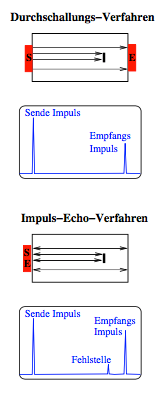
\includegraphics[width=3cm]{bilder/verfahren.png}
  \caption{Durchschallungs- und Impuls-Echo-Verfahren \cite{us2}}
  \label{fig:verfahren}
\end{wrapfigure}
Beim Durchschallungsverfahren wird ein Sender und ein Empfänger benutzt, um den
Körper zu durchstrahlen. Fehlstellen machen sich durch eine abgeschwächte
Intensität bemerkbar, jedoch kann keine Aussage darüber getroffen werden, wo
sich die Fehlstelle befindet.

\noindent Beim Impuls-Echo-Verfahren wird der Sender gleichezeitig auch als Empfänger benutzt,
da der Schall an Grenzflächen reflektiert wird. Bei Fehlstellen ist die Höhe des
Echos für die Größe der Fehlstelle entscheidend. Die Lage der Fehlstelle lässt sich
durch
\begin{equation}
  s = \frac{1}{2} c t
\end{equation}
bestimmen. Diese Laufzeitdiagramme können auf drei verschiedene Arten dargestellt werden.
Zum einen mit einem eindimensionalen Amplituden-Scan (A-Scan) bei dem die Echoamplituden als Funktion
der Laufzeit dargestellt werden. Zum anderen mit einem zweidimensionalen Brightness
Scan (B-Scan) bei dem die Echoamplituden in Helligkeitsabstufungen dargestellt werden.
Die Sonde wird dabei bewegt, um das zweidimensionale Bild zu erzeugen.
Zuletzt gibt es den Time-Motion-Scan (TM-Scan) bei dem durch eine schnelle Abtastung
verschiedene Bewegungen sichtbar gemacht werden können.
